\chapter{NEEM-Hub}
\label{ch:neemhub}
\chapterauthor{S. Koralewski}


Our CRC aims to acquire a huge amount of data, make the data accessible to the research community,  allow to analyze the data, create machine learning models from the data and support version control for the data and models. 
With our \neemhub concept we are covering all those requirements with one system.

To implement the version control of large data sets and machine learning models, we are using DVC\footnote{\url{https://dvc.org/}}. 
We use Hadoop\footnote{\url{https://hadoop.apache.org/}} and its file system HDFS to store the data and models.
Hadoop is a cluster system which creates automatically replicas of the data once it is uploaded and allows parallel processing of data to speed up transforming or querying the data.

On a high level perspective we want to realize two pipelines with our \neemhub as depict in Figure \ref{fig:neem-hub}.
The first pipeline can be seen as the acquisition and analytic pipeline.
The first step in the pipline is storing raw data, such as videos, text, images and electrocardiogram (ECG) data.
In the next step, so called neemifier are transforming this raw data into \neems which are utilizing the semantically representation provided by \soma.
Since we are using Hadoop, multiple instances of the same neemifier can neemify the raw data in parallel. 
There is also the possibility to upload \neems directly to the \neemhub, so the neemifing step can be skipped.
The stored \neems can be accessed by \openease. 
\openease allows the inspection and visualization of each individual \neem.
A direct download of the \neems to a local system is also supported.

The second pipeline should be used as a pipeline for learning from the acquired data.
\neems are so rich full on information that one \neem can be used for multiple learning problems.
In addition, \neems allow to generate models with different levels of abstraction. 
One can learn general models e.g.\ the likely location of perishable items or/and specialized models e.g. how an agent should grasp my favorite mug in my kitchen.
The procedure to generate the models is that transformers are used to extract the required features from the \neems and store them in a data representation, e.g.\ CSV, required for the machine learning model.
The learners, which create the models, store the data in the model library. 
This model library can be used afterwards by an agent to perform reasoning.

In some scenarios those two pipelines can be combined to create a closed-loop. 
A possible scenario can be a robot acquiring \neems, uploading them to the \neemhub and download afterwards the new models to improve itself for the next experiment. 


\begin{figure}[h!]
	\centering
	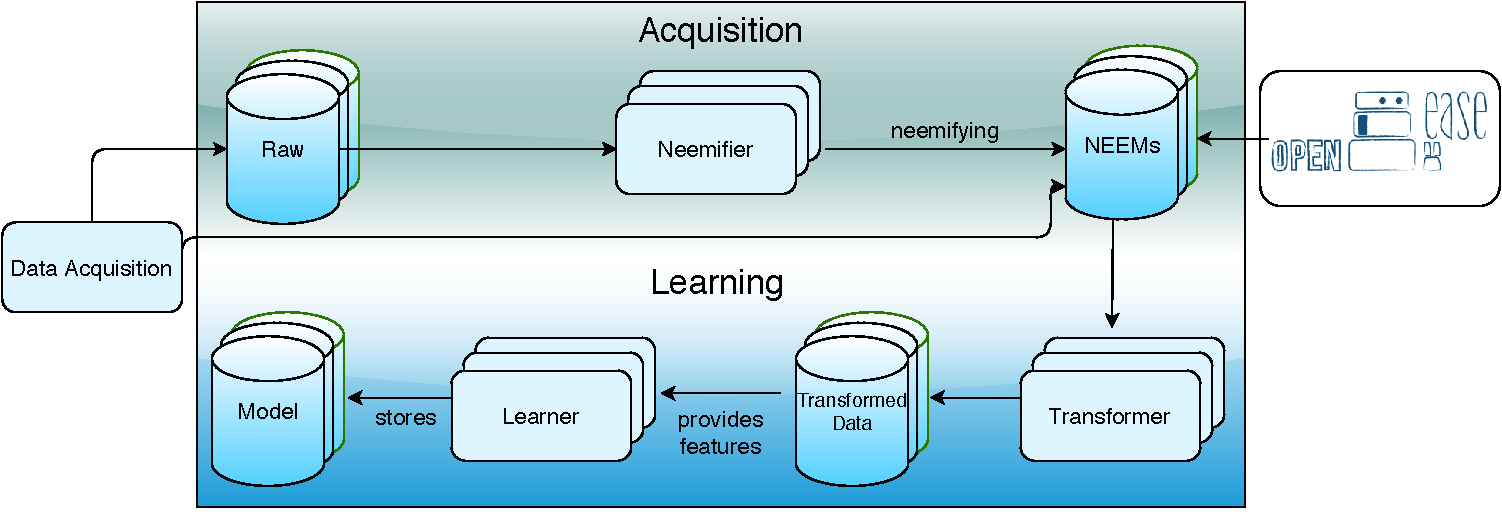
\includegraphics[width=\linewidth]{img/NEEM-Hub.pdf}
	\caption{The NEEM-Hub Architecture}
	\label{fig:neem-hub}
\end{figure} 


Currently, we are only supporting data upload and hosting, like raw data, \neems and transformed data.
In future, we will provide the feature to share your neemifier and transformers with the community and create your own pipelines directly on the \neemhub.
In the rest of this section we will describe how you can upload the data to the \neemhub.

\section{Prerequisite}
\begin{enumerate}
	\item Due to security reasons our Hadoop cluster can be only accessed via the university's intranet right now.	
	\item To support version control with our \neems we have the Install DVC \url{https://dvc.org/} and get familiar with the tool \url{https://dvc.org/doc/start}.
	\item Install Hadoop or a client which can interact with our HDFS filesystem. 
	\item To be able to publish your data, you are required to have a git account on our GitLab system
	\url{https://neemgit.informatik.uni-bremen.de} .
	\item To test if you setup your system successful, you can try to download the following \neems : \url{https://neemgit.informatik.uni-bremen.de/neems/ease-2020-pr2-setting-up-table} .
\end{enumerate}


\section{Publishing}
To organized the raw and transformed data and the \neems, we created 3 groups on GitLab.
Each group corresponds to the specific data set type.
The general procedure to publish your data set is that you create a git repository in the corresponding group.
For instance, if you want to upload a \neem data set, create a repository in the \neem group first.
In the next step, clone the empty repository and initialize DVC in this repository.
Afterwards you need to define the remote storage, to let DVC store your data set.
Based on your data set type you need to use the following path to define the storage:
 
\begin{description}
	\item[\textbf{Raw data}]\leavevmode \newline
		\url{hdfs://hadoop@134.102.137.65:9000/raw/<your-repo-name>}
	\item[\textbf{\neems}] \leavevmode \newline
		\url{hdfs://hadoop@134.102.137.65:9000/neems/<your-repo-name>}
	\item[\textbf{Transformed Data}] \leavevmode \newline
		\url{hdfs://hadoop@134.102.137.65:9000/transformed_data/<your-repo-name>}
\end{description}

In future, you will be able to publish your neemifier and transformers.
This will allow to share your tools easily with the community and also automatize your data transformation and learning pipeline.
